\section{Proposta}
\label{sec:proposta}

\subsection{A aplicação Price Search}

A aplicação Price Search foi pensada com o intuito de facilitar a pesquisa de preço de quaisquer tipos de itens existentes no mercado, sejam eles eletrodomésticos, alimentos, utensílios, remédios, etc. Hoje em dia é possível ncontrar diversos tipos de produtos em \textit{sites} de grandes lojas, porém, como há várias cidades no Brasil que não são atendidas por tais estabelecimentos, percebe-se que há uma grande dificuldade para determinar qual lugar oferece tal produto com o menor custo. Com isso, a ideia da aplicação é que as pessoas tenham acesso a um recurso para comparação de preço dos produtos dos estabelecimentos locais, a fim de ajudar as pessoas a economizar dinheiro. 

Outra finalidade da aplicação é ajudar na busca de produtos, dos quais anteriormente não se sabia onde eram vendidos. Com uma simples pesquisa, o usuário pode identificar facilmente o valor desses produtos e onde encontrá-los, por meio de um mapa que fornece a localização do estabelecimento contendo o seu endereço. 

O intuito é criar uma ferramenta simples, de fácil uso e multiplataforma, com o objetivo de agregar a quantidade máxima de usuários possíveis, para que todos possam usá-la de maneira rápida e eficiente.

\subsection{CRUD}
No projeto há \textit{CRUDs} (do inglês, \textit{Create, Read, Update \& Delete}) que irão realizar operações básicas como criação, recuperação, atualização ou remoção das informações persistidas no banco de dados, como produtos, listas de compras, ofertas, estabelecimentos e usuários. 

\subsection{Progressive Web App}

O \textit{PWA} é uma metodologia de desenvolvimento de aplicações \textit{web} que também se comportem como aplicações nativas, de modo que sua concepção seja facilitada. Ela utiliza \textit{service workers}, que são \textit{scripts} que fazem o gerenciamento do \textit{cache}\footnote{Memória temporária comumente utilizada para armazenar recursos frequentemente acessados por processos.}, fornecendo um melhor desempenho pois os dados e boa parte do \textit{front-end} são persistidos no próprio dispositivo; isso faz com que, em alguns casos, seja possível utilizar a aplicação de forma totalmente \textit{off-line}.

Mesmo sendo uma aplicação \textit{web}, o \textit{PWA} pode acessar grande parte dos recursos do dispositivo, como câmera, \textit{GPS} (do inglês, \textit{Global Positioning System}) e contatos, podendo, portanto, ser usada de forma dinâmica.

Diferentemente dos aplicativos que devem ser baixados de uma loja, a única coisa que o usuário precisa fazer é entrar no \textit{site} da aplicação \textit{web} e, caso tenha interesse, pode salva-la em seu dispositivo, como se fosse uma aplicação móvel. Inclusive, o Google Play Store\footnote{Loja de aplicativos voltada para dispositivos móveis Android. Disponível em \url{https://play.google.com/store}} também se abriu para aplicações \textit{PWA}, tornando sua distribuição retrocompatível com o método convencional.


\subsection{Diagrama de Blocos}

 O diagrama de blocos (ilustrado na Figura  \ref{fig:diagrama_de_blocos}) é uma representação gráfica de todas as tecnologias que foram utilizadas no desenvolvimento do projeto, bem como sobre como é feita a comunicação entre elas.
 
\begin{figure}[!htb]
\centering
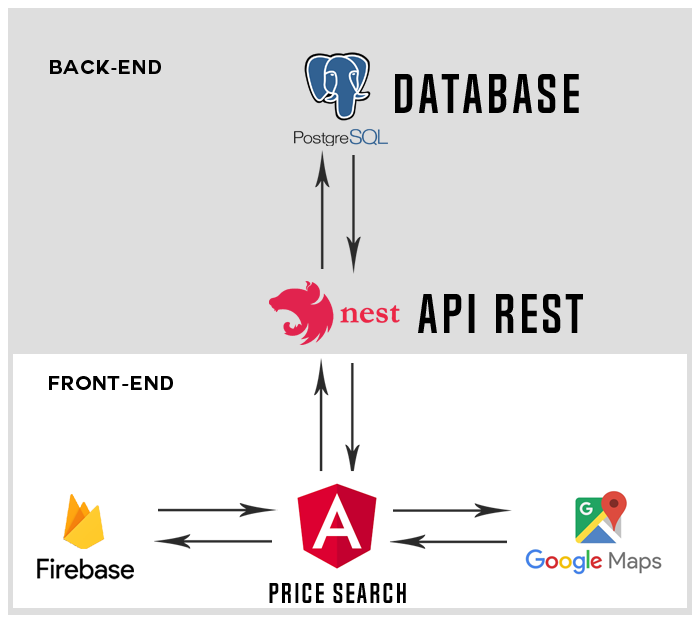
\includegraphics[width=\linewidth]{figuras/diagrama_de_blocos.png}
\caption{Diagrama de blocos da aplicação Price Search.}
\label{fig:diagrama_de_blocos}
\end{figure}
 
 No projeto foi utilizado PostgreSQL como banco de dados, Node.js e REST (do inglês, \textit{Representational State Transfer}\footnote{Princípios ou regras que, quando seguidas, permitem a criação de um projeto com interfaces bem definidas \cite{pires2017rest}.}. A aplicação foi feita utilizando Angular, e foram utilizados o Firebase para autenticação de usuário e a Plataforma Google Maps\footnote{Google Maps Platform é o conjunto de ferramentas necessárias para integrar as funcionalidades do Google Maps em uma aplicação. Disponível em: \url{https://cloud.google.com/maps-platform}} para localização dos estabelecimentos, conforme explicado na seção \ref{sec:ferramentas}.
 
\subsection{Modelo de Dados}
 
 O MER (Modelo Entidade Relacionamento) mostra como os objetos e características de um modelo de negócios se relacionam entre si. De forma geral, o MER descreve como um banco de dados da aplicação é estruturado, ilustrado na Figura \ref{fig:mer}.
 
 
\begin{figure}[!htb]
\centering
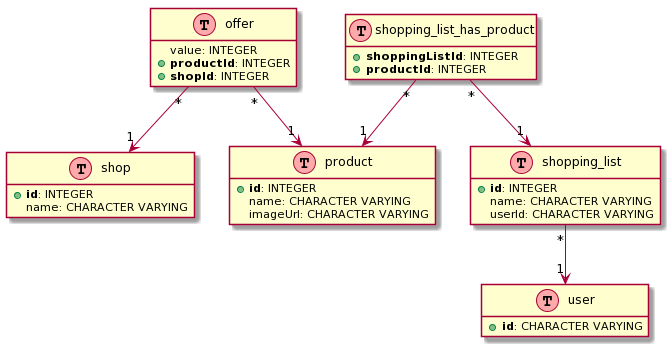
\includegraphics[width=\linewidth]{figuras/MER.png}
\caption{MER da aplicação Price Search.}
\label{fig:mer}
\end{figure}
 
  
 \subsection{Casos de Uso}
O diagrama de casos de uso da aplicação ilustra as ações de um usuário, que tem acesso às funcionalidades listadas, conforme ilustrado na Figura \ref{fig:casos-de-uso}.

\begin{figure}[!htb]
\centering
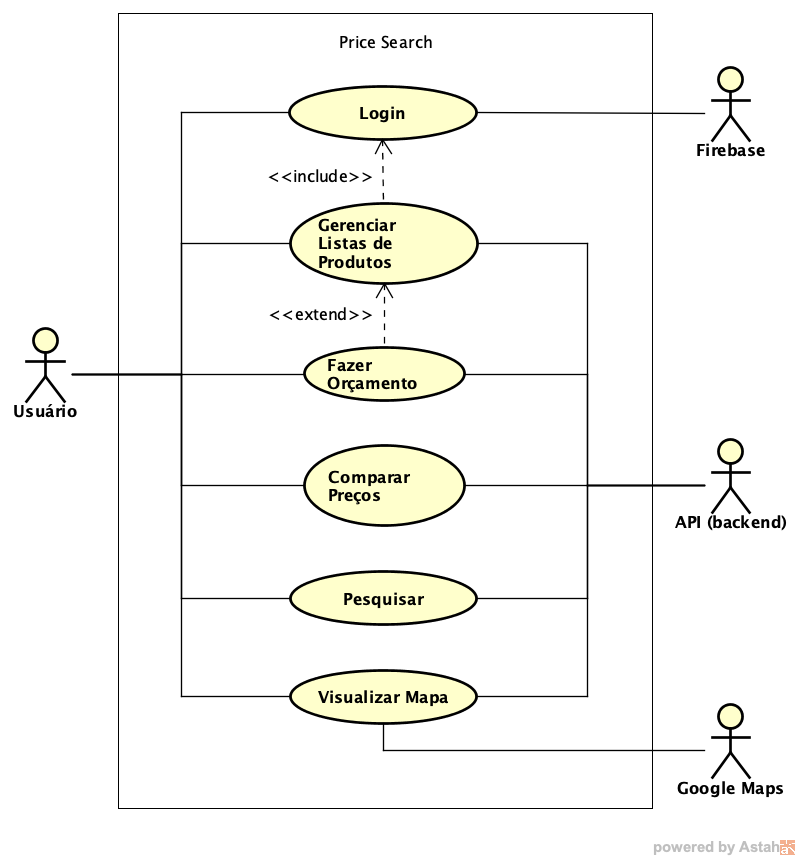
\includegraphics[width=\linewidth]{figuras/DiagramaCasosUsoPriceSearch.png}
\caption{Diagrama de Casos de Uso do Price Search.}
\label{fig:casos-de-uso}
\end{figure}

\subsubsection{Caso de Uso 01: \textit{Login}}

O usuário inicia o \textit{login} (ilustrado na Figura \ref{fig:login}) utilizando uma conta existente do Google, não sendo necessário preenchimento de nenhum tipo de dado pessoal. Feito isto, o assistente valida os dados do usuário e o \textit{login} é efetuado. A aplicação utiliza o ``token'' fornecido pela conta do Google, que é salvo no banco de dados para a sincronização das informações do usuário.

\begin{figure}[H]
\centering
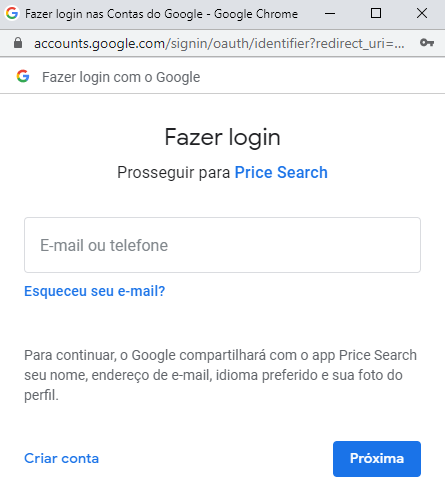
\includegraphics[width=\linewidth]{figuras/tela-login.png}
\caption{Ilustração do Caso de Uso 01: \textit{Login}.}
\label{fig:login}
\end{figure}

\subsubsection{Caso de Uso 02: Pesquisar}

A barra de pesquisa se encontra no topo da página (ilustrado na Figura \ref{fig:menu}); junto dela também existe um botão de menu para mostrar todas as abas do aplicativo. A pesquisa é feita utilizando o nome do produto, então o usuário pode pesquisar por qualquer item, desde que este esteja no banco de dados, e o sistema então retornará todos os itens de acordo com a pesquisa feita realizada.

\begin{figure}[H]
\centering
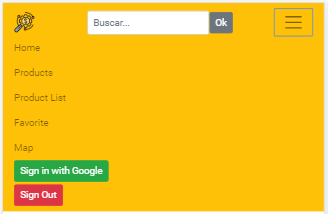
\includegraphics[width=\linewidth]{figuras/tela-menu.png}
\caption{Ilustração do Caso de Uso 02: Pesquisar.}
\label{fig:menu}
\end{figure}

\subsubsection{Caso de Uso 03: Gerenciar Lista de Compra}

O usuário pode criar várias listas de compras, como se fosse um carrinho de compras (ilustrado na Figura \ref{fig:lista}). Ao criar uma lista, o usuário pode escolher um nome para ela, bem como escolher quais itens serão adicionados futuramente e removê-los a qualquer momento, ou mesmo renomear ou excluir a lista.

\begin{figure}[H]
\centering
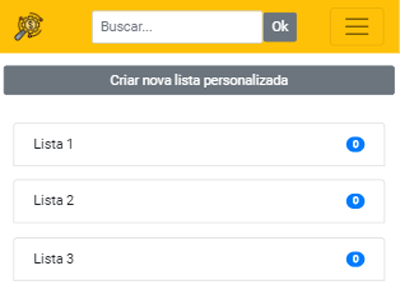
\includegraphics[width=\linewidth]{figuras/tela_lista_personalizada.png}
\caption{Ilustração do Caso de Uso 03: Gerenciar Lista de Compra.}
\label{fig:lista}
\end{figure}

\subsubsection{Caso de Uso 04: Comparar Preços}

O usuário pode comparar preços de um produto em diferentes estabelecimentos (ilustrado na Figura  \ref{fig:comparar}) e, por meio do aplicativo, descobrir em qual estabelecimento ele pode encontrar o melhor preço do produto que deseja.

\begin{figure}[H]
\centering
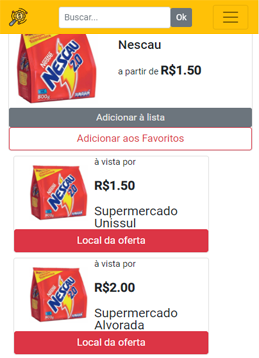
\includegraphics[width=\linewidth]{figuras/tela-comparar.png}
\caption{Ilustração do Caso de Uso 04: Comparar Preços.}
\label{fig:comparar}
\end{figure}

\subsubsection{Caso de Uso 05: Visualizar Mapa}

O usuário tem acesso a um mapa que contém a localização de todos os estabelecimentos locais cadastrados (ilustrado na Figura \ref{fig:mapa}). Ao clicar nos estabelecimentos mostrados no mapa, são fornecidas informações sobre ele, tais como nome e endereço.

\begin{figure}[H]
\centering
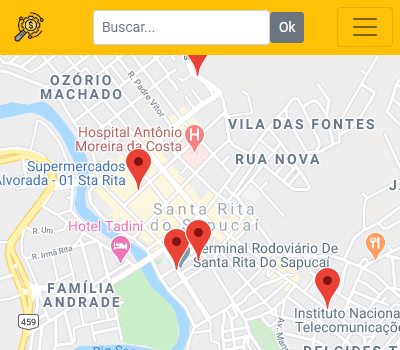
\includegraphics[width=\linewidth]{figuras/tela_mapa.png}
\caption{Ilustração do Caso de Uso 05: Visualizar Mapa.}
\label{fig:mapa}
\end{figure}
